\chapter{Introduction}

%Being a vital organ, the heart is of paramount importance in keeping a human being alive. Therefore, it is necessary to identify anomalies as fast and accurate as possible, to ensure quick and adequate treatment. A straightforward method to do this is using the sound waves that the heart produces. A doctor can do this manually using a stethoscope, but to achieve faster and objective data, a microphone array is superior. This project aims to use a microphone array consisting of 6 microphones to locate the heart valves of a patient and possibly give a diagnosis. 
% instructions on p. 83 of the manual state to not include the relevance of heart monitoring

This report describes a system that uses audio signals recorded by a microphone array placed on a human chest to isolate heart sounds. The goal is to enable analysis of sounds produced by certain regions of the heart, while attenuating sounds from other areas. In this project, only the localization of heart sounds is discussed, while the last module used for isolating sounds based on spatial origin is outside the scope of this report. A six-channel digital stethoscope array is used to record the phonocardiogram (PCG), which is the acoustic signal generated by the mechanical activity of the heart.

To realize heart-sound localization, several subsystems are to be designed:
\begin{itemize}
    \item Heart sound modeling: Test data is needed to evaluate the performance of the various subsystems. This can be achieved by modeling the sounds the heart valves produce and simulating the measurement setup.
    \item Pre-processing: This system takes the raw PCG data and processes it so that it can be used further on in the process by other systems.
    \item Localization: This takes the output after the pre-processing and uses various algorithms to determine the locations the heart valves are most likely at. 
\end{itemize}

This system is represented in more detail in a block diagram as shown in Figure \ref{fig:projectblock}. The first step, acquisition, has already been designed and can be used as it is. After the data has been pre-processed, it is inspected for errors and corrected if needed in a GUI (Graphical User Interface). This must be designed too. Then, localization of the sources takes place. Because many parameters can be varied in that step, this is also connected to a GUI, where the user can set the parameters. 


\label{ways_of_testing}
The system is tested in three ways:
\begin{itemize}
    \item Simulation model. This way of testing is used to test whether the systems work as expected in idealized situations. This model also allows to inject noise and small variations into the data to test robustness.
    \item Phantom model. This is a measurement setup to test whether the results match an idealized reality. This is needed because when testing on human subjects, there is no ground truth about where the valves are. This model makes some simplifications because the real human body is far more complex.
    \item Human subjects. The possibility to test the system on a human body is also present. However, the results of this test cannot be verified, it can only be checked if they look plausible.
\end{itemize}
Out of these three, only the Python model has to be implemented. The hardware for the phantom model and the measurements has already been designed and manufactured.

\begin{figure} [H]
    \centering
    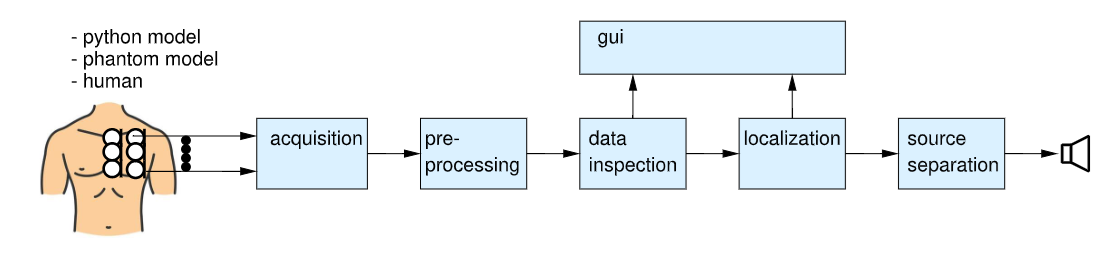
\includegraphics[width=0.60\textwidth]{figures/projectblock.png}
    \caption{Overview of the system, as given in \cite{IP3Man}}  
    \label{fig:projectblock}
\end{figure}

